\chapter{Allgemeines}
\section{Ablauf}

\begin{figure}
	\centering
	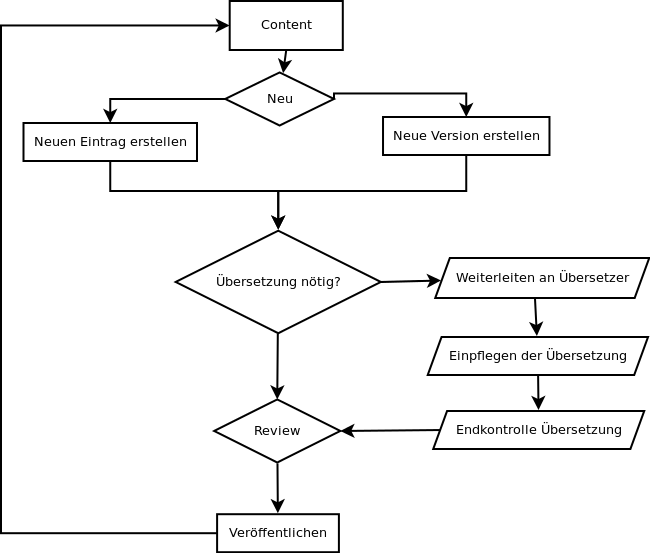
\includegraphics[width=0.75\textwidth]{CMS_Ablaufdiagramm.png}
	\caption{CMS Ablauf}
	\label{CMS Ablauf}
\end{figure}

\section{Men�aufbau}
Der Content kann in hierarchisch angeordnet werden. 
Dadurch ergibt sich die Men�struktur die im CIS verwendet wird.\\

\begin{figure}
	\centering
	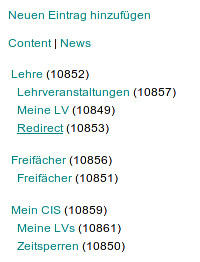
\includegraphics[width=0.30\textwidth]{CMS_Menue.png}
	\caption{CMS Men�struktur}
	\label{CMS Men�struktur}
\end{figure}

\section{Childs}
�ber den Punkt Childs k�nnen die Kindelemente eines Contents zugewiesen werden.
Dadurch wird die Men�struktur definiert. \\
Ein Content darf Child-Element von mehreren Contents sein. (mehrmals im Men�
vorkommen)\\
\\
\section{Zugriffsrechte}
�ber den Punkt Gruppen k�nnen Benutzergruppen zu Seiten zugeordnet werden. 
Nur Benutzer welche sich in diesen Gruppen befinden d�rfen die Seite betrachten.
Wenn keine Gruppe zugeordnet ist, ist die Seite f�r alle sichtbar.\\
Es k�nnen hier nur Gruppen ausgew�hlt werden, bei denen das Attribut Content 
auf true gesetzt ist.

\section{History}
Hier k�nnen die verschiedenen Versionen miteinander verglichen werden. 
Die Unterschiede zueinander werden farblich markiert. 